\documentclass[11pt]{article}

\usepackage[T1]{fontenc}
\usepackage{lmodern}
\usepackage[margin=1in]{geometry}
\usepackage{amsmath,amssymb,amsthm}
\usepackage{microtype}
\usepackage{graphicx}
\usepackage{booktabs}
\usepackage{array}
\usepackage{enumitem}
\usepackage{xcolor}
\usepackage{fancyhdr}
\usepackage[hidelinks]{hyperref}
\hypersetup{
  pdfauthor={Ioannis Tsiokos},
  pdftitle={Six Birds for Neutrino Mass: Lens-Swap Stability and Packaging Audits}
}
\usepackage{cleveref}
\crefname{section}{Section}{Sections}
\crefname{figure}{Figure}{Figures}
\crefname{table}{Table}{Tables}
\crefname{equation}{Eq.}{Eqs.}
\usepackage[numbers,sort&compress]{natbib}
\usepackage{orcidlink}

\graphicspath{{figures/}}

% Operators / notation
\newcommand{\Lens}{f}
\newcommand{\Completion}{U}
\newcommand{\Pack}{E}
\newcommand{\PackageOp}{\mathcal{E}}
\newcommand{\RouteMismatch}{\Delta_{\mathrm{route}}}
\newcommand{\Staging}{\mathrm{staging}}
\newcommand{\dchi}{\Delta \chi^2}
\newcommand{\mnu}{\sum m_\nu}

\numberwithin{equation}{section}

% Prevent widows and orphans
\widowpenalty=10000
\clubpenalty=10000
\raggedbottom

% Affiliation helper (submission-style author block).
\makeatletter
\newcommand{\affiliation}[1]{\gdef\@affiliation{#1}}
\newcommand{\printaffiliation}{\begin{center}\small \@affiliation\end{center}}
\makeatother

\title{Six Birds for Neutrino Mass:\texorpdfstring{\\}{ } Lens-Swap Stability and Packaging Audits}
\author{Ioannis Tsiokos\,\orcidlink{0009-0009-7659-5964}}
\affiliation{}
\date{2 March 2026\\[4pt]{\small Version 1}}

\fancypagestyle{firstpage}{%
  \fancyhf{}
  \fancyfoot[C]{\scriptsize Automorph Inc., Wilmington, DE, USA \quad \texttt{ioannis@automorph.io} \quad \textcopyright\ 2026 \quad CC-BY 4.0 \quad Preprint --- not peer reviewed.}
  \renewcommand{\headrulewidth}{0pt}
  \renewcommand{\footrulewidth}{0pt}
}

\begin{document}

\maketitle
\thispagestyle{firstpage}
\printaffiliation

\begin{abstract}
\label{sec:abstract}
When the SPT-3G 2018 temperature and polarization likelihood is replaced by the later SPT-3G D1 release, which observes essentially the same patch of sky, cosmological upper limits on the summed neutrino mass $\mnu$ have been reported to tighten \cite{arxiv2601_16277}. We ask a prior question: do the two released likelihoods make mutually consistent predictions? Following the Six Birds framework \cite{sixbirds_foundations,sixbirds_darkenergy}, we treat each release as a \emph{lens} on the same sky and measure, in each direction, how much worse one lens fits at parameters chosen by the other. We split the SPT quadratic part of this mismatch across spectra and multipoles with a signed allocation that respects the full covariance, so the pieces add up exactly to that part. At numerically optimized (but not certified-global) fits, the mismatch is large and strongly asymmetric. Testing D1 at the 2018 fit costs $\dchi\approx488$ for SPT with DESI DR2 BAO and $\approx63$ with a Planck-subset baseline added; the reverse direction costs $\approx79$ and $\approx23$. Where the mismatch sits depends on both baseline and direction: temperature at $2000\le\ell<3000$ leads both directions of the SPT+DESI audit, whereas polarization (EE) leads the D1-given-2018 direction once the Planck subset is included. Cutting D1 back to the 2018 multipole coverage, dropping the SPT optical-depth prior, or raising Boltzmann precision changes each tested total by less than 4\%. Our archived single-chain $\mnu$ runs, and a later multi-chain campaign, do not meet pre-declared convergence and precision criteria, and the likelihoods themselves proved sensitive to solver version and numerical settings. We therefore report no tightening magnitude. We also give a short, machine-checked (Lean 4) analysis of two Gaussian constraints with the physical gate $\mnu\ge0$. It shows when the posterior mode sits exactly at zero, that tension between two constraints that both prefer positive masses can never put it there, and that tightening one constraint raises the chance of a boundary mode only when the other constraint's mean is positive.

\end{abstract}

\noindent\textbf{keywords:} neutrino mass; cosmological bounds; SPT-3G; lens stability; cross-lens audit; packaging mismatch; Six Birds framework

\section{Introduction}
\label{sec:intro}

The summed neutrino mass $\mnu$ is one of the main targets of precision cosmology. Its constraints come from combining early-universe information in the cosmic microwave background (CMB) with late-time distance measurements such as baryon acoustic oscillations (BAO). As upper limits approach the minimum allowed by oscillation experiments, a practical question becomes pressing: when a limit moves, how much of the movement reflects the sky, and how much reflects choices in how the data were processed and compressed into a likelihood?

A sharp example is reported in \cite{arxiv2601_16277}. The authors compare two releases of the South Pole Telescope SPT-3G temperature and polarization (TT/TE/EE) likelihood: the 2018 release and the later D1 release built from the 2019--2020 seasons. Holding the rest of their CMB baseline fixed (a subset of Planck 2018 products plus Planck PR4 lensing, together with the matching SPT lensing product), they find that switching from the 2018 to the D1 combination tightens the $\mnu$ upper limit and moves the posterior towards the physical boundary $\mnu=0$. They call the shift ``curious'', because both releases observe essentially the same field, and they point out that the decisive test would be to reprocess the 2018 raw data through the D1 pipeline. We do not claim that test as our idea, and we do not perform it.

\paragraph{The question we ask.}
Before interpreting a parameter shift, one can ask whether the two released likelihoods agree with each other at all. We frame this with the Six Birds framework \cite{sixbirds_foundations,sixbirds_darkenergy}. Each likelihood release is a \emph{lens}: a map from the sky (together with instrument and foreground nuisances) to a likelihood object. Here ``lens'' never means gravitational lensing. A model class with its nuisance parameterization and priors is a \emph{completion}. The posterior we report is the \emph{package} obtained by composing the two. If two lenses describe the same sky consistently, parameters chosen by one should fit the other reasonably well. We measure how far this fails, in each direction separately, and where in the data the failure sits.

\paragraph{What this paper contributes.}
\begin{enumerate}[leftmargin=*, itemsep=2pt]
  \item \textbf{Directional cross-lens audits.} We fit one SPT release (with a common completion), transfer the shared cosmological parameters to the other release, and record the loss in fit relative to that release's own best fit. We do this in both directions, for two baselines (SPT with DESI DR2 BAO, and SPT with a Planck subset, Planck PR4 lensing and DESI), and under three controls: a multipole-support cut, removal of the SPT optical-depth prior, and higher Boltzmann precision (\cref{sec:results-audits}).
  \item \textbf{Exact localization with correlated data.} We split the SPT quadratic part of each mismatch over spectra and multipole bands with a signed allocation that uses the full covariance matrix. The pieces sum exactly to that quadratic part, unlike block-by-block chi-squares, which fail to add up when blocks are correlated; native prior and normalization terms are accounted for separately (\cref{sec:ledger}). The resulting maps show that the location of the mismatch depends on both the baseline and the direction of transfer.
  \item \textbf{A clear statement of what the $\mnu$ chains support.} Our sampled posteriors do not pass convergence and quantile-precision checks fixed in advance, and the likelihood evaluations turned out to be sensitive to solver version and numerical settings. We therefore report no magnitude for the $\mnu$ tightening, and we explain what a qualified claim would require (\cref{sec:results-mnu}).
  \item \textbf{A verified boundary mechanism.} For two Gaussian constraints and the gate $\mnu\ge0$, we state exactly when the posterior mode sits at zero, show that two constraints that both prefer positive masses can never put it there, and show that tightening one constraint can make a boundary mode either more or less likely depending on the other constraint's sign. All statements are checked in Lean~4 with Mathlib \cite{lean4,mathlib} (\cref{sec:boundary-mode} and Appendix~\ref{app:formal}).
\end{enumerate}

\paragraph{What this paper does not claim.}
We do not identify the instrumental or analysis cause of the disagreement, and we do not claim a correct value or bound for $\mnu$. Our audit values come from numerical optimizations that are not certified to be global optima, and they are not calibrated significance tests. The SBT language provides the vocabulary of the audits. It is not a theorem that supplies the missing physical steps.

\paragraph{Outline.}
\Cref{sec:related-work} places the work in context. \Cref{sec:sbt-framework} introduces lenses, packages and the directional audit. \Cref{sec:baselines} defines the data combinations and \cref{sec:methods} the audit and sampling procedures. \Cref{sec:results-audits} presents the audits and \cref{sec:results-mnu} the status of the $\mnu$ posteriors. \Cref{sec:boundary-mode} analyses boundary modes, and \cref{sec:discussion,sec:conclusion} discuss limitations and conclude. The appendices list the formal results, describe reproducibility, and record the version history.

\section{Related work}
\label{sec:related-work}
This note builds on the lens-swap observation in \cite{arxiv2601_16277} and the Six Birds/SBT framing in \cite{sixbirds_foundations,sixbirds_darkenergy}. Our computations use standard cosmology inference and Boltzmann tools \cite{cobaya,class,camb}, DESI DR2 BAO likelihood data \cite{desi_dr2_bao_docs,bao_data_v26}, and Planck products \cite{planck2018_cosmoparams,planck_pr4_lensing}.

\section{Six Birds / SBT framing}
\label{sec:sbt-framework}

We summarize the minimal Six Birds / SBT primitives needed for this note and map them to the SPT2018$\rightarrow$D1 lens swap \cite{sixbirds_foundations,sixbirds_darkenergy}. The role of this section is operational: it explains why a shift in a packaged parameter bound under a pipeline change should be treated as a first-class stability question, and why explicit audits and staging controls are the appropriate response.

\paragraph{Lenses, completions, and packaging.}
A \emph{lens} is any data-processing and compression map that produces an inference object (here: a likelihood) from an underlying microstate. In this paper, a lens is emphatically \emph{not} gravitational lensing; it is a pipeline/likelihood release. Let $X$ denote the relevant microstate (cosmology plus nuisance/systematic degrees of freedom) and let
\begin{equation}
  \Lens : X \to \mathcal{L}
  \label{eq:lens_map}
\end{equation}
denote the map that takes the microstate to a likelihood object (or its sufficient summary). A \emph{completion} specifies how we close the discarded information: a macro-model class, nuisance parameterization, and priors. In our setting, $U$ is $\Lambda$CDM+$\mnu$ with an explicit physical gate $\mnu\ge 0$ and the nuisance/foreground parameterization appropriate to each likelihood release. Packaging is the composition
\begin{equation}
  \Pack \;=\; \Completion \circ \Lens,
  \label{eq:packaging_def}
\end{equation}
which maps the (unobserved) microstate to a packaged macro object such as a posterior distribution or a best-fit point. In the idealized limit of a coherent package, benign changes to the lens (e.g.\ changing observing season or pipeline implementation while viewing the same sky) should not drastically change the packaged macro output.

\paragraph{A directional audit statistic for lens swaps.}
SBT emphasizes that when two lenses disagree, one should quantify the mismatch \emph{directionally} via train/test style audits \cite{sixbirds_darkenergy}. Let $\log \mathcal{L}_A(\theta)$ and $\log \mathcal{L}_B(\theta)$ be the log-likelihoods for two lenses $A$ and $B$ under a shared parameter vector $\theta$. Define the (possibly non-unique) best-fit estimator for each lens,
\begin{equation}
  \hat\theta_{L} \in \arg\max_{\theta}\, \log \mathcal{L}_{L}(\theta), \qquad L\in\{A,B\}.
  \label{eq:theta_hat_def}
\end{equation}
The basic held-out mismatch statistic we use throughout is the directional improvement in $B$ when moving from the $A$-fit to the $B$-fit:
\begin{equation}
  \dchi_{B|A} \;\equiv\; -2\left[\log \mathcal{L}_B(\hat\theta_A) - \log \mathcal{L}_B(\hat\theta_B)\right].
  \label{eq:dchi_def}
\end{equation}
By construction, $\dchi_{B|A}\ge 0$ when $\hat\theta_B$ is the maximizer found by our optimizer/sampler; large $\dchi_{B|A}$ indicates that the $A$-packaged macro object predicts $B$ poorly, even after accounting for $B$'s own internal best-fit. Importantly, $\dchi_{B|A}$ need not equal $\dchi_{A|B}$: route mismatch is typically \emph{directional}. When the likelihood supports blockwise decomposition (e.g.\ by spectrum and multipole band), $\dchi_{B|A}$ can be localized as a sum of per-block contributions, turning an abstract mismatch into a concrete ``where to look'' diagnostic.

\paragraph{Staging and common-support controls.}
SBT distinguishes intrinsic lens mismatch from artifacts of \emph{staging}---changes in effective resolution, smoothing, cuts, or support that can change the packaged object even under perfect internal consistency \cite{sixbirds_foundations}. In CMB likelihoods, multipole cuts are a primary staging control. When comparing SPT2018 and SPT D1, we therefore implement a \emph{common-staging} control in which the D1 likelihood is restricted (as much as feasible) to the SPT2018 multipole support, and we repeat the same directional audits. If mismatch persists under common-staging and remains localized inside the overlap region, the evidence points away from simple support/cut explanations.

\paragraph{Six Birds primitives (P1--P6) in this note.}
Table~\ref{tab:sixbirds_primitives} summarizes the primitives and their instantiation here. The table is not meant to be exhaustive; it is a compact guide to the audit logic used in the remainder of the paper.

\begin{table}[t]
  \centering
  \caption{Six Birds primitives (P1--P6) and their instantiation in the SPT2018$\leftrightarrow$D1 lens swap setting.}
  \label{tab:sixbirds_primitives}
  \setlength{\tabcolsep}{4pt}
  \renewcommand{\arraystretch}{1.08}
  \small
  \begin{tabular}{@{}>{\raggedright\arraybackslash}p{0.16\linewidth} >{\raggedright\arraybackslash}p{0.28\linewidth} >{\raggedright\arraybackslash}p{0.50\linewidth}@{}}
    \toprule
    Primitive & SBT meaning (informal) & Instantiation in this work \\
    \midrule
    \textbf{P1 Rewrite} &
    Minimal correction needed for macro closure when packaged dynamics fail to commute &
    We treat boundary sensitivity as a generic truncation effect under mismatch; \emph{in a toy-only demonstration}, a one-mode surrogate rewrite reduces cross-lens $\dchi$ without invoking new physics. We do not apply a rewrite-mode correction to the real SPT lens swap in this note. \\
    \textbf{P2 Gating} &
    Constraints defining admissible macro objects and completions &
    Physical gate $\mnu\ge 0$; dataset inclusion/exclusion (e.g.\ no Planck high-$\ell$ TE/EE); nuisance parameterization choices. \\
    \textbf{P3 Route mismatch} &
    Non-commutation / staging dependence of packaged outputs across routes &
    The lens swap $A=\text{SPT2018}$ vs $B=\text{SPT D1}$ yields different packaged inferences; we quantify route mismatch via directional $\dchi_{B|A}$ and $\dchi_{A|B}$. \\
    \textbf{P4 Staging} &
    Dependence on scale, resolution, support, or cut choices &
    Common-staging control by matching multipole support across lenses; we test whether the mismatch is explained by $\ell$-range differences. \\
    \textbf{P5 Packaging} &
    The packaged macro object produced by $(\Completion\circ\Lens)$ &
    Posteriors/best-fits for $\mnu$ and nuisance parameters are treated as packaged objects; instability under lens swap is a packaging-stability failure. \\
    \textbf{P6 Accounting / audit} &
    Held-out prediction and decomposition of failures &
    Cross-lens audits and localization by spectrum and multipole provide an actionable diagnosis of where the packaged summaries disagree. \\
    \bottomrule
  \end{tabular}
\end{table}

\paragraph{Mapping to the inconsistency.}
In the remainder of the paper, we treat the two SPT likelihood releases as two lenses on (nearly) the same sky. The question is not ``which lens is correct,'' but whether a packaged inference is \emph{stable} under this lens change. When it is not, SBT prescribes two immediate steps: (i) quantify and localize mismatch via audits (\cref{eq:dchi_def}), and (ii) test whether staging controls eliminate the mismatch. Only after these checks does it become meaningful to interpret parameter-level shifts---including $\mnu$ tightening or boundary motion---as potentially cosmological rather than packaging-sensitive.

\section{Data sets and baselines}
\label{sec:baselines}

Our goal is to isolate the effect of swapping one CMB \emph{lens} for another while holding fixed, as much as feasible, the rest of the ``baseline'' structure emphasized in \cite{arxiv2601_16277}. Throughout, we treat likelihood releases as lenses (pipeline likelihood objects), not as immutable ground truth. This section defines the two SPT lenses and the baseline dataset combinations used later for both audits and $\mnu$ inference.

\subsection{SPT-3G lenses: 2018 vs D1}
\label{sec:spt-lenses}

We work with two SPT-3G multifrequency TT/TE/EE likelihood releases, treated as distinct lenses and evaluated through \texttt{candl} \cite{candl}:
\begin{itemize}[leftmargin=*, itemsep=2pt]
  \item \textbf{SPT2018 lens:} SPT-3G 2018 TT/TE/EE likelihood \cite{spt3g2018_ttteee}\\
    (Candl ID \texttt{candl\_data.SPT3G\_2018\_TTTEEE\_multifreq}).\\
    The effective multipole ranges are TT $750\le \ell\le 3000$ and TE/EE $300\le \ell\le 3000$.
  \item \textbf{SPT D1 lens:} SPT-3G D1 (2019--2020) TT/TE/EE likelihood \cite{spt3g_d1}\\
    (Candl ID \texttt{spt\_candl\_data.SPT3G\_D1\_TnE\_multifreq}).\\
    The effective multipole ranges are TT $400\le \ell\le 3000$ and TE/EE $400\le \ell\le 4000$.
\end{itemize}
These definitions and ranges follow the baseline description in \cite{arxiv2601_16277}.

\subsection{Planck subset and PR4 lensing baseline}
\label{sec:planck-subset}

To match the structure of the ``CMB baseline'' used in \cite{arxiv2601_16277}, we implement a Planck PR3 subset together with Planck PR4 lensing \cite{planck2018_likelihood}:
\begin{itemize}[leftmargin=*, itemsep=2pt]
  \item \textbf{Low-$\ell$ Planck PR3:} TT for $\ell<30$ and EE for $\ell<30$ (we use the \texttt{EE\_sroll2} variant available in Cobaya's Planck likelihood family).
  \item \textbf{Truncated high-$\ell$ Planck PR3 TT:} TT only for $30\le \ell\le 756$ via \texttt{planck\_2018\_highl\_plik.\allowbreak TT\_lite\_native} with \texttt{bins\_for\_L\_range=\allowbreak[30,756]}.
  \item \textbf{No Planck high-$\ell$ TE/EE:} in accordance with \cite{arxiv2601_16277}, we do not include high-$\ell$ Planck TE/EE likelihoods.
  \item \textbf{Planck PR4 lensing:} we include the public PR4 (NPIPE) lensing likelihood \cite{planck_pr4_lensing,planck_pr4_lensing_maps} via
    \texttt{planckpr4lensing.PlanckPR4Lensing}.
\end{itemize}
We emphasize that this is an operational baseline intended to match the selection described in \cite{arxiv2601_16277}; it is not the full Planck 2018 likelihood \cite{planck2018_cosmoparams}.

A compact summary of the two CMB baselines used throughout is given in Table~\ref{tab:baseline-defs}.

\begin{table}[t]
  \centering
  \caption{Baseline definitions as described in \cite{arxiv2601_16277} (CMB and CMB-D1). In our implementation we match the Planck-subset + PR4 lensing structure and swap only the SPT TT/TE/EE likelihood release; see text for any deviations.}
  \label{tab:baseline-defs}
  \small
  \begin{tabular}{@{} p{0.13\linewidth} p{0.28\linewidth} p{0.33\linewidth} p{0.18\linewidth} @{}}
\toprule
Baseline & SPT primary ($\ell$ ranges) & Planck PR3 primary subset & Lensing \\
\midrule
CMB (SPT2018) & TT $[\ell_{\min},\ell_{\max}]{=}[750,3000]$; TE/EE $[\ell_{\min},\ell_{\max}]{=}[300,3000]$ & TT $\ell<30$ (Commander); EE $\ell<30$ (SRoll2); TT $30<\ell<756$ (Plik). & SPT lensing + Planck PR4 lensing \\
CMB-D1 & TT $[\ell_{\min},\ell_{\max}]{=}[400,3000]$; TE/EE $[\ell_{\min},\ell_{\max}]{=}[400,4000]$ & TT $\ell<30$ (Commander); EE $\ell<30$ (SRoll2); TT $30<\ell<756$ (Plik). & SPT lensing + Planck PR4 lensing \\
\bottomrule
\end{tabular}

\end{table}

Implementation note: our runs use the released SPT TT/TE/EE likelihood objects for SPT2018 and D1, together with the Planck subset and Planck PR4 lensing. We do not include a separate SPT lensing-reconstruction likelihood component. Therefore, our ``Planck-subset baseline'' should be read as matching the Planck selection in \cite{arxiv2601_16277} while only partially matching their CMB baseline composition; this is a plausible contributor to residual numerical differences in $\mnu$ bounds.

\subsection{DESI DR2 BAO likelihood}
\label{sec:desi-bao}

For BAO, we implement a Gaussian likelihood for DESI DR2 BAO using the publicly documented DR2 BAO mean vectors and covariance matrices \cite{desi_dr2_bao_docs,bao_data_v26,desi_dr2_results_ii_bao,desi_dr2_results_i_lya}. The implemented observable vector includes $(D_M/r_d)$, $(D_H/r_d)$, and $(D_V/r_d)$ points from the DR2 Gaussian BAO compression for the ``ALL'' combined set \cite{desi_dr2_bao_docs,bao_data_v26,eisenstein2005_baopeak}. This combined set includes low-redshift galaxy BAO and Ly$\alpha$ forest BAO points, so our ``ALL'' vector is not purely galaxy BAO. Theory predictions are computed from the same cosmological backend used for CMB inference (\cref{sec:mnu-inference}).

\subsection{Non-novelty note: pipeline reprocessing diagnostic}
\label{sec:non-novelty}

The baseline-swap sensitivity highlighted in \cite{arxiv2601_16277} naturally motivates a decisive diagnostic: reprocessing the 2018 raw data through the D1 pipeline to separate sky information from pipeline effects. We explicitly acknowledge that this diagnostic is already emphasized in \cite{arxiv2601_16277}; we do not claim novelty for proposing it. Our focus here is complementary: we provide a packaging/audit framework and a set of concrete, localizable metrics that quantify and stage-control the lens mismatch in the packaged likelihood objects available today.

\section{Methods}
\label{sec:methods}

This section summarizes (i) the audit metrics used to quantify and localize cross-lens mismatch, (ii) the common-staging control, and (iii) the cosmological inference setup used to estimate $\mnu$ posteriors in the presence of lens swaps.

\subsection{Directional cross-lens audits and localization}
\label{sec:audit-metrics}

Our primary audit statistic is the directional held-out mismatch $\dchi_{B|A}$ defined in \cref{eq:dchi_def}. Intuitively, $\dchi_{B|A}$ asks: if we package the macro object using lens $A$, how poorly does that packaged solution predict lens $B$ relative to $B$'s own internal best fit? Because route mismatch is directional, we report both $\dchi_{B|A}$ and $\dchi_{A|B}$.

When the likelihood supports blockwise decomposition (e.g.\ by spectrum and multipole band), we additionally localize mismatch by writing $\dchi_{B|A}$ as a sum over blocks. In our implementation, blocks correspond to a spectrum type (TT/TE/EE) and an $\ell$-bin group. The result is a heatmap-style diagnostic that turns a global mismatch into a concrete localization: which spectrum and which multipole ranges dominate the held-out failure.

\paragraph{Blockwise accounting.}
When a likelihood provides additive blockwise contributions (e.g.\ by spectrum and multipole groups), we write
\begin{equation}
  \log \mathcal{L}_B(\theta) \;=\; \sum_{g\in\mathcal{G}} \log \mathcal{L}_{B,g}(\theta),
  \label{eq:block_decomp}
\end{equation}
and define the blockwise held-out mismatch contributions
\begin{equation}
  \dchi_{B|A,g} \;\equiv\; -2\left[\log \mathcal{L}_{B,g}(\hat\theta_A) - \log \mathcal{L}_{B,g}(\hat\theta_B)\right].
  \label{eq:block_dchi}
\end{equation}
Under \cref{eq:block_decomp} these satisfy the sum rule $\dchi_{B|A}=\sum_{g\in\mathcal{G}}\dchi_{B|A,g}$ (and similarly for $A|B$), so the localization heatmaps should be read as an accounting decomposition of the same directional audit statistic rather than an unrelated diagnostic.
We emphasize that $\dchi$ is reported in the native $-2\Delta\log\mathcal{L}$ units of the packaged likelihood objects and is used here as a comparative diagnostic (across directions and staging controls), not as a calibrated hypothesis-test p-value; null calibration would require additional held-out or posterior-predictive constructions beyond the scope of this short note.

\subsection{Profiled audits: separating shared parameters from nuisance packaging}
\label{sec:profiled-audit}

A key subtlety is that lenses can differ in nuisance parameterization and calibration degrees of freedom. To more closely align the audit with SBT's ``completion'' semantics, we also implement a \emph{profiled} variant of the cross-lens audit. For direction $B|A$, we:
\begin{enumerate}[leftmargin=*, itemsep=2pt]
  \item hold fixed a small set of \emph{shared} parameters (the intersection of parameters we choose to treat as common across lenses), and
  \item re-optimize a tractable subset of $B$'s nuisance parameters (a calibration/bandpower-mode subset) to maximize $\log \mathcal{L}_B$ under those shared parameters.
\end{enumerate}
We then compute a profiled $\dchi_{B|A}$ by comparing $B$'s likelihood at the profiled $A$-shared point against $B$'s own profiled best fit. Operationally, this separates (i) mismatch that can be absorbed by lens-specific nuisance packaging from (ii) mismatch that persists even after giving the test lens freedom to retune its nuisance degrees of freedom.

In practice, full profiling over all nuisance parameters can be computationally expensive. We therefore use a runtime-capped profiling set consisting of a calibration/beta subset (referred to internally as \texttt{TT\_cal\_beta}), reduced to a tractable number of parameters for deterministic optimization.
\paragraph{Formal definition.}
Let parameters be partitioned as $\theta=(\phi,\eta_B)$ where $\phi$ denotes the shared parameters we hold fixed in the audit direction $B|A$ and $\eta_B$ denotes nuisance parameters specific to lens $B$. Define the profiled log-likelihood
\begin{equation}
  \log \widetilde{\mathcal{L}}_B(\phi) \;\equiv\; \max_{\eta_B}\, \log \mathcal{L}_B(\phi,\eta_B),
  \label{eq:profile_loglike}
\end{equation}
and the profiled directional mismatch
\begin{equation}
  \widetilde{\dchi}_{B|A} \;\equiv\; -2\left[\log \widetilde{\mathcal{L}}_B(\hat\phi_A) - \log \widetilde{\mathcal{L}}_B(\hat\phi_B)\right],
  \label{eq:profile_dchi}
\end{equation}
where $\hat\phi_L$ is the shared-parameter component of the best-fit point under lens $L$.
In practice we approximate \cref{eq:profile_loglike} by profiling only a tractable subset of $B$'s nuisance parameters under a runtime cap; the intent is not to ``profile away'' all mismatch, but to reduce sensitivity to purely lens-specific packaging degrees of freedom.
In our implementation, the profiled set comprises the following calibration/beta parameters:
\begin{quote}\small\raggedright
\texttt{Tcal\_ext150},
\texttt{Tcal\_rel90},
\texttt{Tcal\_rel220},
\texttt{Ecal\_ext150},
\texttt{Ecal\_rel90},
\texttt{Ecal\_rel220},
\texttt{TT\_CIBClustering\_Alpha},
\texttt{TT\_CIB\_150x150},
\texttt{TT\_CIB\_150x220},
\texttt{TT\_CIB\_220x220},
\texttt{TT\_GalCirrus\_Alpha},
\texttt{TT\_GalCirrus\_Amp}.
\end{quote}
\noindent For the reverse direction, the capped set is:
\begin{quote}\small\raggedright
\texttt{TT\_tSZ\_CIB\_Corr\_Amp},
\texttt{TT\_tSZ\_CIB\_corr},
\texttt{Ecal150},
\texttt{Ecal220},
\texttt{Ecal90},
\texttt{TT\_CIBClustering\_Alpha},
\texttt{TT\_CIBClustering\_Amp},
\texttt{TT\_CIBClustering\_Beta},
\texttt{TT\_GalCirrus\_Alpha},
\texttt{TT\_GalCirrus\_Amp},
\texttt{TT\_GalCirrus\_Beta},
\texttt{TT\_Poisson\_150x150}
\end{quote}
\noindent (runtime-capped to 12 parameters; see run metadata).

\subsection{Common-staging control}
\label{sec:common-staging}

Because the two SPT lenses differ in multipole support, a basic staging control is to restrict the broader-support lens to the narrower-support range and repeat the same audits. We implement a \emph{common-staging} control in which the D1 lens is restricted (as much as feasible) to the SPT2018 multipole support (TT: $\ell\ge 750$; TE/EE: $\ell\ge 300$; all with $\ell\le 3000$). The restriction is implemented at likelihood-instantiation time via selection masks recorded in the run metadata. If mismatch persists under common-staging and remains localized inside the overlap region, this points away from a pure support/cut explanation.
This common-staging control matches \emph{multipole support} but does not fully equalize the compressed summaries: the two releases retain their own bandpower binning/window functions and internal covariance conventions, so this test should be interpreted as a support/cut control rather than an identity-of-data-vector comparison.

\subsection{$\mnu$ inference pipeline}
\label{sec:mnu-inference}

We estimate $\mnu$ posteriors using Cobaya \cite{cobaya} with a standard Boltzmann backend (CLASS \cite{class} and/or CAMB \cite{camb}, depending on the configuration). The canonical SPT-only+DESI results use \textbf{CAMB} while the Planck-subset baseline+DESI results use \textbf{CLASS}; see run metadata for exact configs. We sample the standard six $\Lambda$CDM parameters $\{\omega_b h^2, \omega_c h^2, H_0, \ln(10^{10}A_s), n_s, \tau\}$ together with $\mnu$ under a physical gate $\mnu\ge 0$. Following the neutrino modeling description in \cite{arxiv2601_16277}, our $\Lambda$CDM+$\mnu$ completion assumes three degenerate massive neutrino states when $\mnu$ is allowed to vary.

\paragraph{Implementation caveat (CLASS parameterization).}
CLASS expects massive neutrinos to be specified via $N_{\mathrm{ncdm}}$ and per-species masses $m_{\mathrm{ncdm}}$. To keep $\mnu$ explicitly present in the recorded chains and summaries while providing CLASS the required per-species masses, we sample an internal parameter (denoted \texttt{mnu\_sample}) and define a derived parameter $\mnu$ together with $m_{\mathrm{ncdm}}=(\mnu/3,\mnu/3,\mnu/3)$. This is a parameterization workaround; it preserves the reported $\mnu$ posterior but should be kept in mind when comparing config syntax to other pipelines.

\paragraph{Priors and stability checks.}
The lower bound $\mnu\ge 0$ is explicit in \cite{arxiv2601_16277}. The upper bound of the prior is not stated in the paper source we audited; for reproducibility we therefore use a broad flat prior with upper bound $5\,\mathrm{eV}$ and report this choice explicitly. Since the resulting posteriors and 95\% upper bounds we report are all $\ll 1,\mathrm{eV}$, this upper bound is not active in practice; the relevant gate for boundary behavior is the physical constraint $\mnu\ge 0$. For each production run we record basic chain diagnostics (split-$\hat R$ \cite{gelman_rubin1992,vehtari2021_rhat} and a crude ESS estimate \cite{vehtari2021_rhat} for $\mnu$) and a half-chain stability proxy for the 95\% upper bound. We also perform a mild stability check by repeating (or partially re-running) one production configuration with a distinct random seed and verifying that the 95\% upper bound does not change materially.
Posterior summaries (quantiles, KDE-based 1D densities, and simple convergence heuristics) are computed using GetDist \cite{getdist}.

\subsection{Reproducibility note}
\label{sec:reproducibility}

All results in this note are tied to canonical run bundles recorded in \path{docs/findings/freeze_checklist.md} and summarized in \path{docs/findings/canonical_results.json}.
All figures and tables appearing in the paper are curated from, or auto-generated against, canonical run bundles and a canonical results summary, so the numerical claims in the text are backed by a deterministic artifact pipeline rather than manual transcription.
The full analysis code, experiment runners, and manuscript build workflow are available at \url{https://github.com/ioannist/six-birds-neutrino}.
The figures curated under \path{paper/figures/} and the tables under \path{paper/tables/} are generated from these canonical artifacts. For convenience, the primary run bundles cited later include:
\begin{itemize}[leftmargin=*, itemsep=2pt]
  \item SPT-only + DESI $\mnu$ shift comparison: \path{runs/20260212_080120_648405_mnu_shift_spt_only_desi}.
  \item Planck-subset baseline + DESI $\mnu$ shift comparison: \path{runs/20260212_111357_576743_mnu_shift_cmb_plancksubset_desi}.
  \item Profiled baseline vs common-staging audit comparison: \path{runs/20260211_181258_958327_spt_profiled_common_staging_compare}.
\end{itemize}
A one-command rebuild of key artifacts is provided by \texttt{make freeze\_check}, and the neutrino inference workflows are exposed via \texttt{make mnu\_smoke} and \texttt{make mnu\_full} when required external assets are present.

\section{Audit results: lens mismatch, localization, and staging}
\label{sec:results-audits}

We now treat the SPT2018 likelihood and the SPT D1 likelihood as two \emph{lenses} on (nearly) the same sky field. The central question is whether packaged outputs are stable under swapping these lenses. Following \cref{eq:dchi_def}, we quantify stability via directional held-out mismatch statistics and then localize the mismatch by spectrum and multipole.

\subsection{Directional mismatch is large and asymmetric}
Table~\ref{tab:audit-summary} summarizes the directional cross-lens audit statistics for both the \emph{unprofiled} audit (evaluating each lens at the other lens's best-fit point) and the \emph{profiled} audit (re-optimizing a tractable subset of the test lens's nuisance parameters; \cref{sec:profiled-audit}). Two qualitative features are immediate:
\begin{enumerate}[leftmargin=*, itemsep=2pt]
  \item \textbf{Mismatch is directional.} The values of $\dchi_{B|A}$ and $\dchi_{A|B}$ differ substantially, indicating that route mismatch is not symmetric across the two lenses.
  \item \textbf{Mismatch is large even after profiling.} Profiling reduces sensitivity to purely lens-specific nuisance packaging, but does not eliminate the held-out failure, indicating that the mismatch is not solely a matter of nuisance retuning.
\end{enumerate}

\begin{table}[t]
  \centering
  \caption{Directional cross-lens audit summary for SPT2018 vs SPT D1, with and without common-staging. The unprofiled audit uses direct evaluation of the test lens at the train lens's best-fit point; the profiled audit re-optimizes a tractable subset of test-lens nuisance parameters at fixed shared parameters (\cref{sec:profiled-audit}). ``Common-staging'' restricts the D1 lens to the SPT2018 multipole support (\cref{sec:common-staging}).}
  \label{tab:audit-summary}
  \resizebox{\linewidth}{!}{\begin{tabular}{@{}l l r r@{}}
\toprule
Audit scope & Variant & $\dchi_{\mathrm{D1}|2018}$ & $\dchi_{2018|\mathrm{D1}}$ \\
\midrule
SPT only, fixed spectra & nuisance-profiled & 849.63 & 414.39 \\
 & + support cut & 837.15 & 415.79 \\
\addlinespace
SPT + DESI & baseline & 488.30 & 79.13 \\
 & + support cut & 486.61 & 80.52 \\
\addlinespace
Full CMB + DESI & baseline (multistart) & 62.59 & 23.17 \\
 & baseline (warm start) & 62.39 & 23.19 \\
 & + support cut & 64.62 & 23.39 \\
 & $-$ SPT $\tau$ prior & 61.28 & 23.11 \\
 & + CLASS precision & 61.39 & 23.08 \\
\bottomrule
\end{tabular}
}
\end{table}

\subsection{Localization points to TT high-$\ell$ structure in the overlap region}
To make the mismatch actionable, we localize $\dchi$ by decomposing it into contributions grouped by spectrum type and multipole ranges. Figure~\ref{fig:profiled-localization} shows the resulting localization heatmaps for the \emph{profiled} audit in both directions. The dominant contributions arise from TT at high multipoles (notably the $\ell\sim 2000$--$3000$ range), while TE/EE contributions are comparatively small.
Because high-$\ell$ TT is foreground- and calibration-sensitive, this localization should be read as identifying where the \emph{packaged likelihood objects} disagree (e.g., foreground modeling, calibration/beam/transfer-function conventions, or covariance structure), not as a map-level diagnosis of the sky.

A key observation is that these multipoles lie well \emph{inside} the overlap region of the two SPT lenses. In other words, the mismatch is not primarily driven by the fact that D1 extends to lower $\ell$ in TT or to higher $\ell$ in TE/EE. Rather, the held-out failure is concentrated in TT structure that both lenses nominally cover. This localization supports interpreting the ``curious shift'' highlighted in \cite{arxiv2601_16277} as a packaging stability failure tied to how the two lenses compress and model the same underlying sky information.

\begin{figure}[t]
  \centering
  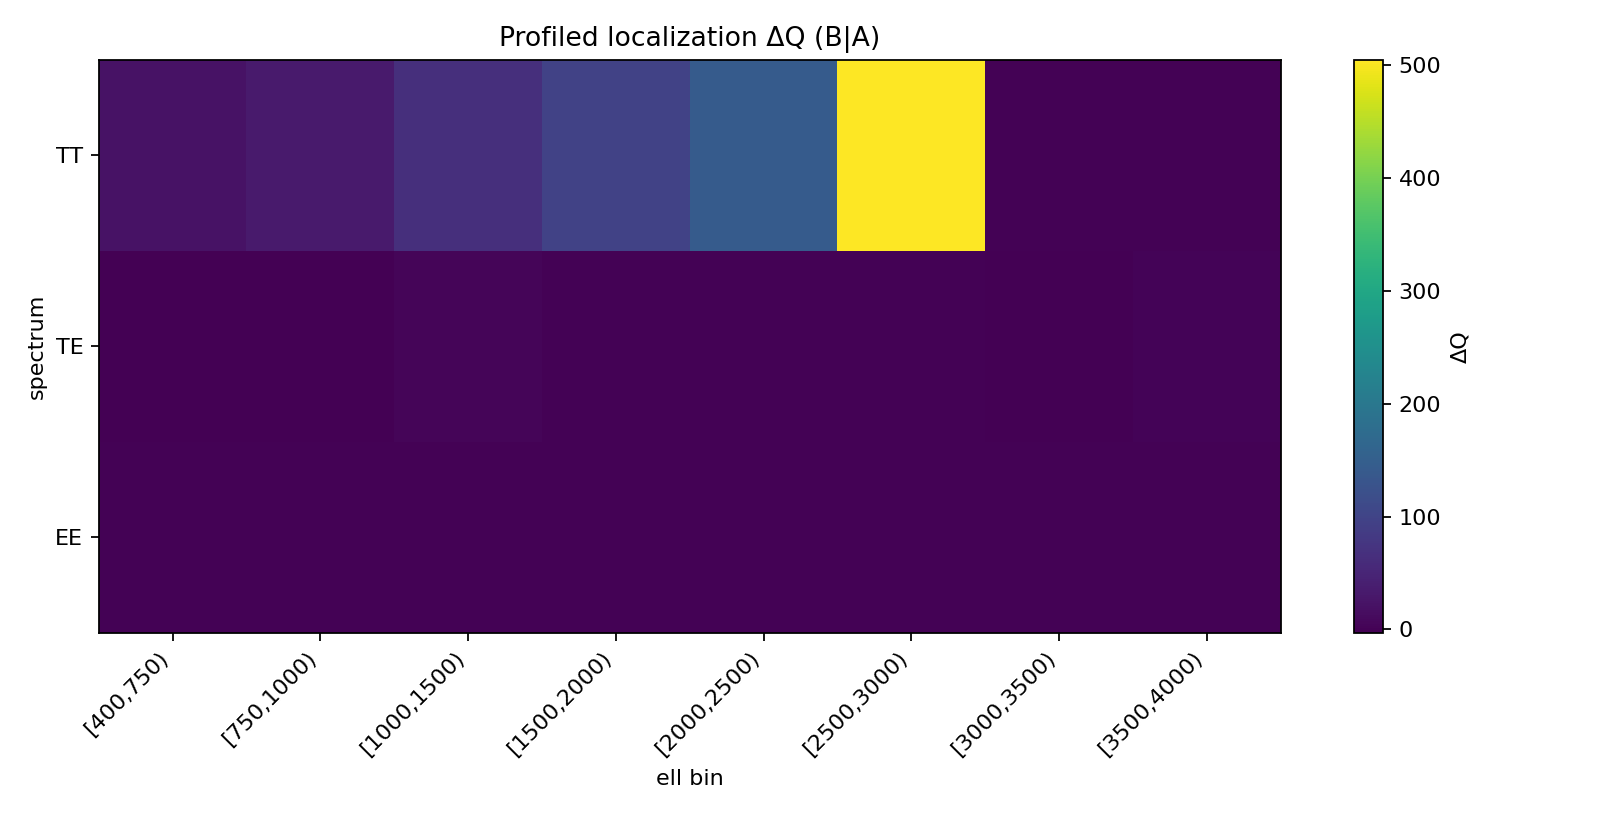
\includegraphics[width=0.49\linewidth]{figures/fig_profiled_localization_B_given_A.png}
  \hfill
  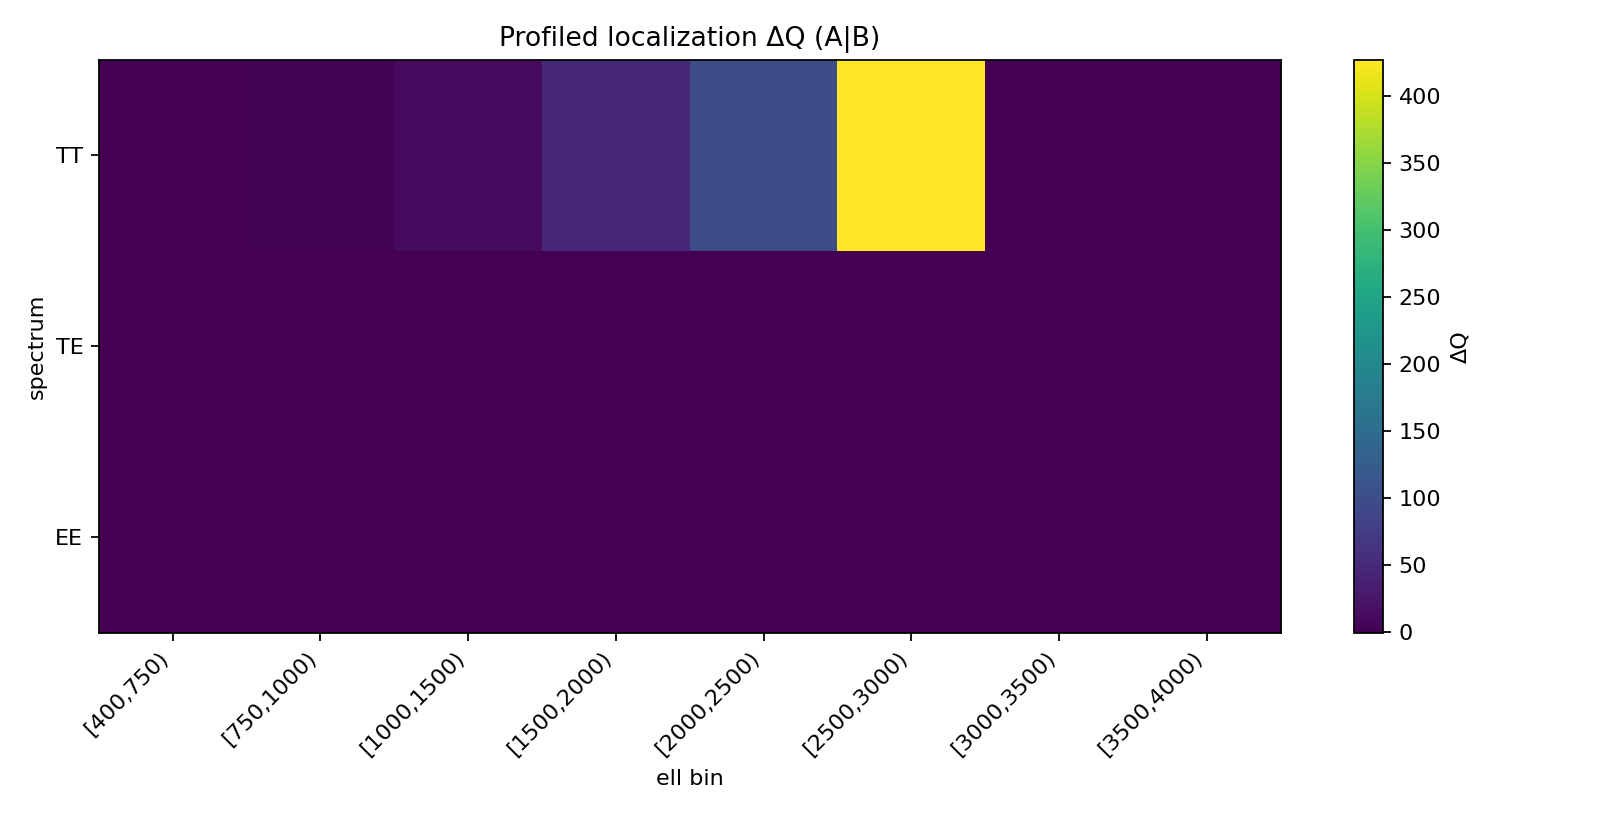
\includegraphics[width=0.49\linewidth]{figures/fig_profiled_localization_A_given_B.png}
  \caption{Profiled localization heatmaps for the SPT lens swap, decomposing the directional held-out mismatch into contributions grouped by spectrum type and multipole ranges. \textbf{Left:} $\dchi_{B|A}$ (SPT D1 given SPT2018). \textbf{Right:} $\dchi_{A|B}$ (SPT2018 given SPT D1). Darker regions indicate larger contributions to the held-out failure. In both directions, the dominant contributions arise from TT at high multipoles within the overlap region.}
  \label{fig:profiled-localization}
\end{figure}

\subsection{Common-staging changes mismatch only at the few-percent level}
A natural hypothesis is that the mismatch is driven by differences in multipole support between SPT2018 and D1. To test this, we implement a common-staging control in which the D1 lens is restricted (as much as feasible) to the SPT2018 multipole support and we repeat the same audits (\cref{sec:common-staging}).

Figure~\ref{fig:profiled-staging-compare} visualizes the baseline-vs-common-staging comparison for the \emph{profiled} audit. The resulting changes are modest: common-staging does not qualitatively resolve the mismatch, and the localization remains dominated by TT high-$\ell$ structure within the overlap region. This control therefore argues against a purely support/cut explanation for the lens mismatch and motivates treating parameter-level shifts (including $\mnu$ tightening) as packaging-sensitive unless accompanied by explicit lens-swap audits.

\begin{figure}[t]
  \centering
  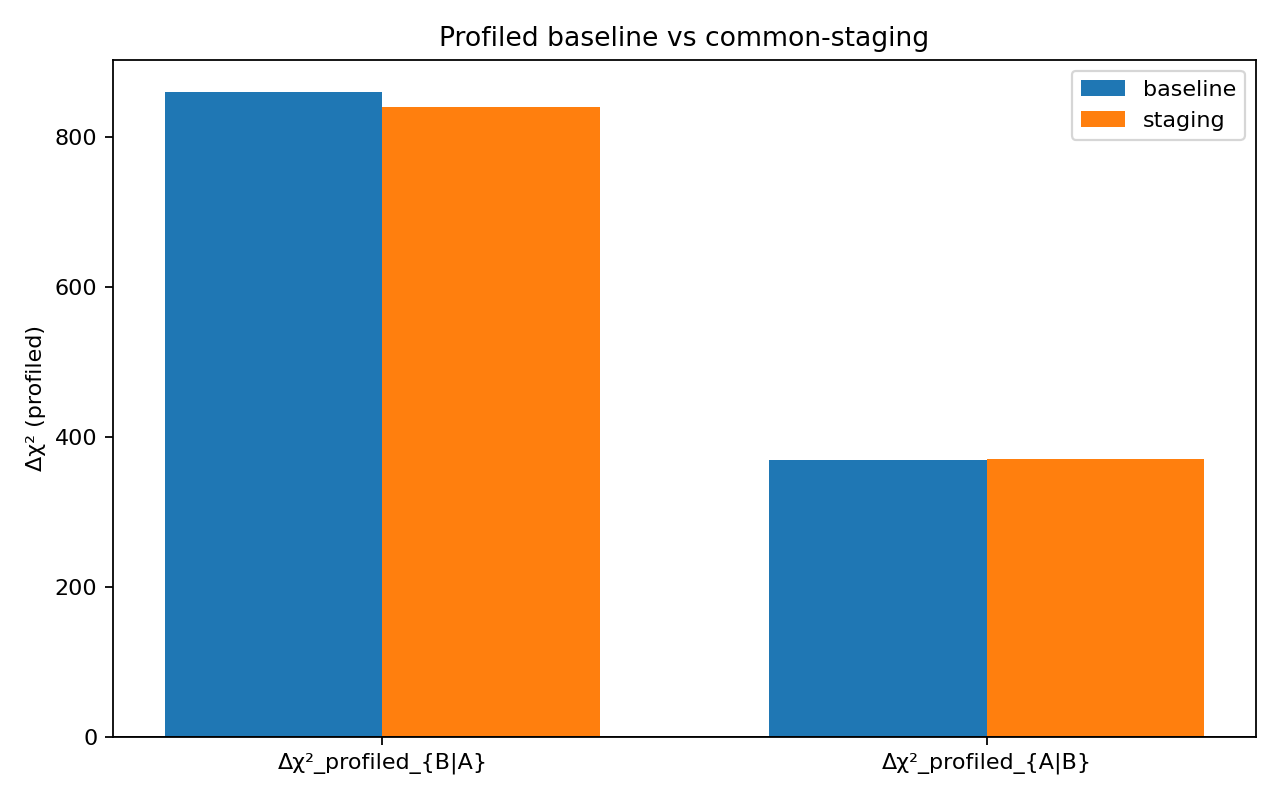
\includegraphics[width=0.85\linewidth]{figures/fig_profiled_staging_compare.png}
  \caption{Common-staging control for the profiled cross-lens audit. Baseline uses the full D1 multipole support; common-staging restricts D1 to the SPT2018 support. The change in $\dchi$ is small compared to the overall mismatch, indicating that staging alone does not explain the held-out failures.}
  \label{fig:profiled-staging-compare}
\end{figure}

\section{Results: $\mnu$ shift under a lens swap}
\label{sec:results-mnu}

We now report the $\mnu$-posterior shifts induced by swapping the SPT lens (SPT2018 $\rightarrow$ SPT D1) under a fixed completion (\cref{sec:mnu-inference}). We emphasize the intended interpretation: these shifts are \emph{packaged} outputs and should be read alongside the lens-swap audits in \cref{sec:results-audits}, which localize where the two lenses disagree and test whether staging controls resolve the mismatch.

\begin{table}[t]
  \centering
  \caption{Summary of $\mnu$ shifts reproduced in this note. Values are in eV; ``Shift'' denotes (SPT2018 minus SPT D1) for the corresponding setup.}
  \label{tab:mnu-shift}
  \resizebox{\linewidth}{!}{\begin{tabular}{l l r r r r}
\toprule
Setup & Lens & median [eV] & 95\% upper [eV] & mode [eV] & boundary frac \\
\midrule
\multicolumn{6}{l}{\emph{SPT-only + DESI DR2 BAO}} \\
 & SPT2018 & 0.071 & 0.194 & 0.050 & 0.00223 \\
 & SPT D1 & 0.042 & 0.085 & 0.070 & 0 \\
 & Shift (2018 $-$ D1) & 0.029 & 0.109 & --- & --- \\
\addlinespace
\multicolumn{6}{l}{\emph{Planck-subset baseline + PR4 lensing + SPT + DESI DR2 BAO}} \\
 & SPT2018 baseline & 0.068 & 0.080 & 0.075 & 0 \\
 & SPT D1 baseline & 0.054 & 0.068 & 0.054 & 0 \\
 & Shift (2018 $-$ D1) & 0.013 & 0.012 & --- & --- \\
\bottomrule
\end{tabular}
}
\end{table}

\subsection{SPT-only + DESI DR2 BAO: a large tightening under D1}
We first consider an intentionally simplified regime: the SPT TT/TE/EE likelihood alone (SPT2018 or D1) combined with DESI DR2 BAO. This setting is useful because it isolates the effect of swapping the SPT lens while holding fixed the late-time distance information. As summarized in Table~\ref{tab:mnu-shift}, the D1 lens yields a substantially tighter $\mnu$ upper bound than the 2018 lens in this regime.

Figure~\ref{fig:mnu-overlay-spt-desi} overlays the $\mnu$ posteriors for this SPT-only+DESI comparison. The qualitative effect is robust: under the same BAO likelihood and completion class, swapping SPT2018$\rightarrow$D1 tightens $\mnu$.

\begin{figure}[t]
  \centering
  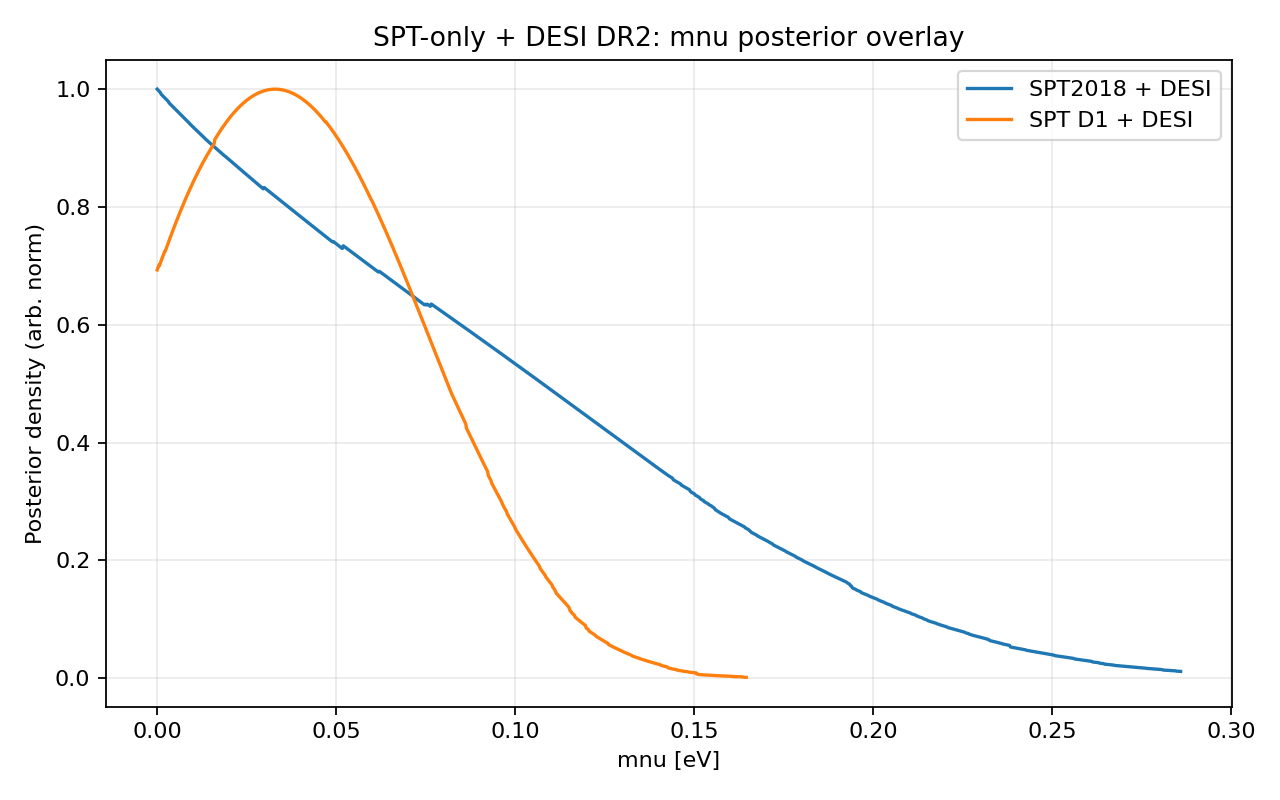
\includegraphics[width=0.85\linewidth]{figures/fig_mnu_overlay_spt_desi.png}
  \caption{$\mnu$ posterior overlay for SPT-only + DESI DR2 BAO. The D1 lens yields a tighter $\mnu$ constraint than the SPT2018 lens under the same BAO likelihood and completion. Numerical summaries are given in Table~\ref{tab:mnu-shift}.}
  \label{fig:mnu-overlay-spt-desi}
\end{figure}

\subsection{Planck-subset baseline + PR4 lensing + DESI: headline replication with a smaller shift}
We next run a baseline designed to mirror the Planck-subset+PR4-lensing structure described in \cite{arxiv2601_16277} (\cref{sec:planck-subset}), and we again combine with DESI DR2 BAO. In this setting the \emph{direction} of the lens-swap effect matches the headline behavior emphasized in \cite{arxiv2601_16277}: swapping SPT2018$\rightarrow$D1 tightens the $\mnu$ upper bound. However, the magnitude of the tightening in our reproduction is smaller than the difference between the corresponding values quoted in \cite{arxiv2601_16277} (Table~\ref{tab:mnu-shift}).
Because this baseline shift is at the $\mathcal{O}(10^{-2},\mathrm{eV})$ level, we treat it as a \emph{directional} replication: its magnitude is comparable to our seed-based stability proxy for the 95\% upper bound, so we avoid over-interpreting small numerical differences.

Figure~\ref{fig:mnu-plancksubset-desi} shows the $\mnu$ posterior overlay for this baseline+DESI setting together with a compact bounds summary table. In these production runs we do not observe strong posterior piling at the physical boundary $\mnu=0$ (the boundary-fraction diagnostic is near zero), but a boundary mode can arise generically under truncation when inconsistent packaged constraints are tightened; we return to this mechanism in \cref{sec:boundary-mode}.

\begin{figure}[t]
  \centering
  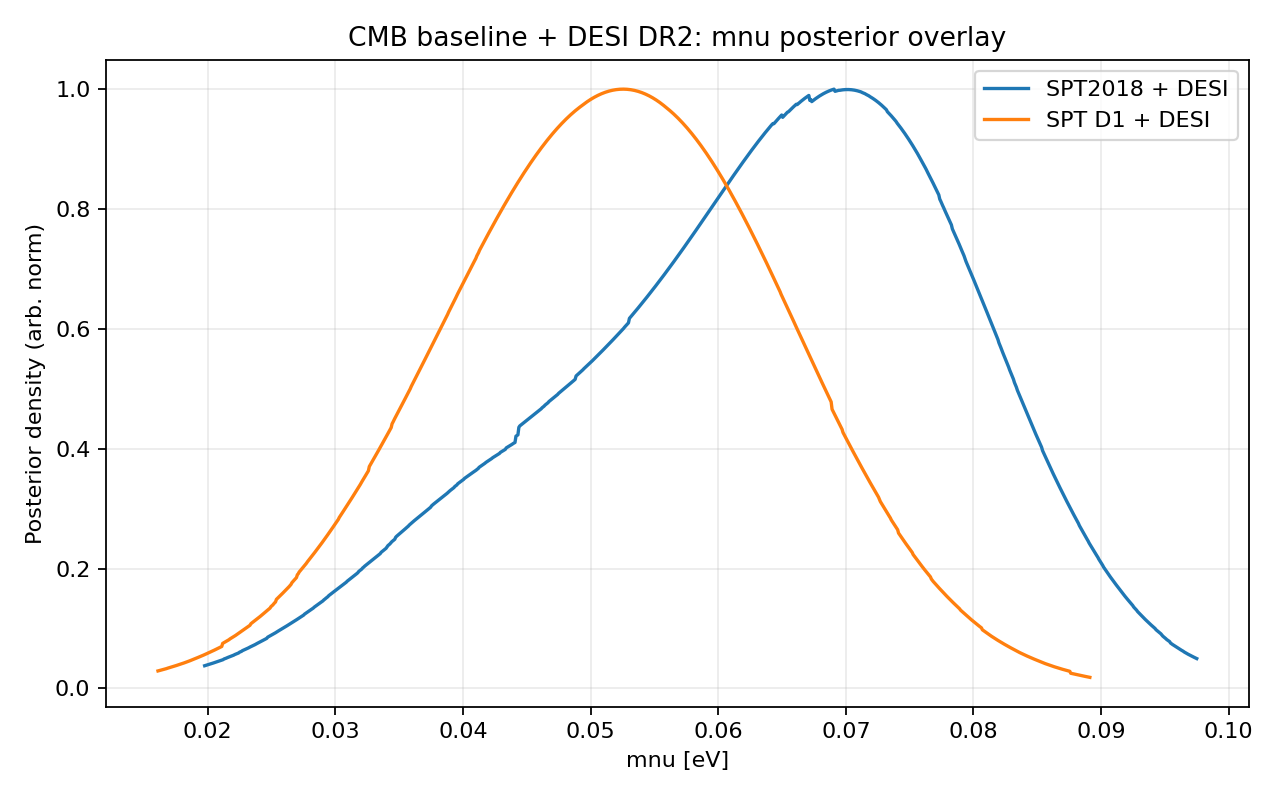
\includegraphics[width=0.85\linewidth]{figures/fig_mnu_overlay_plancksubset_desi.png}

  \vspace{6pt}
  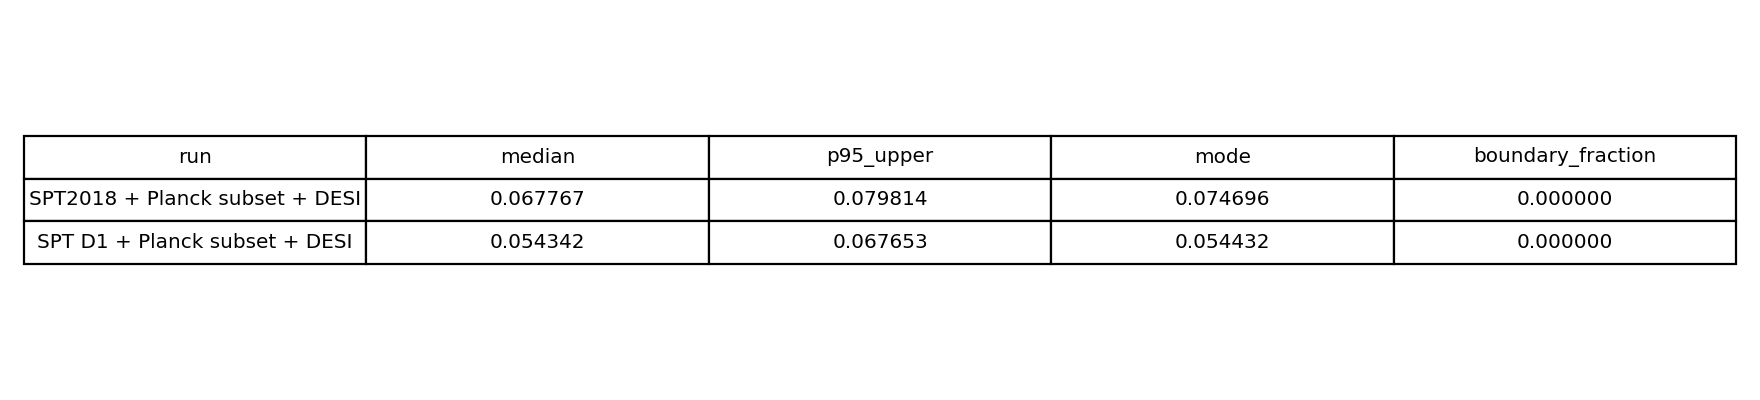
\includegraphics[width=0.85\linewidth]{figures/fig_mnu_bounds_plancksubset_desi.png}
  \caption{$\mnu$ posterior overlay (top) and bounds summary (bottom) for the Planck-subset baseline + PR4 lensing + SPT + DESI DR2 BAO setting. The D1 lens again yields a tighter $\mnu$ constraint than SPT2018, but the shift magnitude is smaller than the gap reported in \cite{arxiv2601_16277}. See Table~\ref{tab:mnu-shift} for the numerical comparison.}
  \label{fig:mnu-plancksubset-desi}
\end{figure}

\subsection{Comparison to \cite{arxiv2601_16277} and likely drivers of residual differences}
For context, \cite{arxiv2601_16277} reports 95\% upper bounds of $\mnu<0.11\,\mathrm{eV}$ for their SPT2018-based CMB baseline + DESI DR2 BAO, and $\mnu<0.069\,\mathrm{eV}$ for the corresponding CMB-D1 baseline + DESI DR2 BAO.
Our reproduction matches the \emph{direction} highlighted in \cite{arxiv2601_16277}: under DESI DR2 BAO, swapping SPT2018$\rightarrow$D1 tightens the $\mnu$ upper bound. The \emph{magnitude} of the shift depends on details of the completion and likelihood packaging. Several plausible contributors to the remaining numerical differences (particularly in the SPT2018 baseline bound) include:
\begin{itemize}[leftmargin=*, itemsep=2pt]
  \item \textbf{Nuisance freedom and priors.} We use a deliberately minimal nuisance sampling set for computational tractability in production chains; tighter or looser bounds can result when additional nuisance parameters are varied, reparameterized, or assigned different priors.
  \item \textbf{Planck low-$\ell$ EE variant.} Our Planck subset uses the \texttt{EE\_sroll2} low-$\ell$ EE likelihood variant available in Cobaya; small baseline differences can propagate into tight derived bounds.
  \item \textbf{Likelihood and pipeline versions.} Even when dataset selections are conceptually matched, differences in released likelihood implementations, calibration conventions, and default settings can shift posteriors in the sub-0.1\,eV regime.
  \item \textbf{Baseline components.} Our baseline matches the Planck-subset and PR4 lensing structure described in \cite{arxiv2601_16277}, but exact numerical agreement can depend on whether additional baseline components (and their nuisance couplings) are included and how they are parameterized in a given code stack.
  \item \textbf{SPT lensing component.} The CMB baseline in \cite{arxiv2601_16277} includes an SPT lensing-reconstruction likelihood component; our baseline implementation does not, which can affect absolute tight bounds and may reduce the shift magnitude.
\end{itemize}
These sensitivities are precisely why we advocate pairing headline parameter bounds with explicit lens-swap audits and staging controls (\cref{sec:results-audits}): when the packaged likelihood objects disagree in localized regions of the summary statistics, parameter-level shifts should be interpreted as packaging-sensitive until the mismatch is resolved.

\subsection{Implementation caveat: sampled \texttt{mnu\_sample} and derived $\mnu$}
\label{sec:mnu-impl-caveat}
As noted in \cref{sec:mnu-inference}, our Planck-subset baseline production runs are CLASS-based and parameterize massive neutrinos via three degenerate species masses $m_{\mathrm{ncdm}}=(\mnu/3,\mnu/3,\mnu/3)$. To keep $\mnu$ explicit in chain outputs while providing CLASS the required per-species masses, we sample an internal parameter \texttt{mnu\_sample} and expose $\mnu$ as a derived parameter used for reporting and plotting. This is a bookkeeping choice for tool compatibility; it does not change the intended meaning of the reported $\mnu$ posterior.

\section{Boundary modes under a physical gate}
\label{sec:boundary-mode}

The authors of \cite{arxiv2601_16277} report that with D1 the $\mnu$ posterior is pushed against the prior border at $\mnu=0$. This section asks, in the simplest possible model, when such boundary behavior arises and how it responds to tightening. Every proposition below is proved in Lean~4 with Mathlib. Appendix~\ref{app:formal} maps each statement to its formal counterpart. The model assumes exactly Gaussian, independent constraints and, for posterior statements, a prior that is constant on the allowed region. These are assumptions of the model, and we have not shown that real CMB or BAO likelihoods satisfy them.

\subsection{Two Gaussian constraints and a gate}
Let $m\ge0$ stand for $\mnu$. Two independent constraints contribute Gaussian factors $\exp[-(m-\mu_i)^2/(2\sigma_i^2)]$ with $\sigma_i>0$ and precisions $a=\sigma_1^{-2}$, $b=\sigma_2^{-2}$. Completing the square gives
\begin{equation}
  a(m-\mu_1)^2+b(m-\mu_2)^2 \;=\; (a+b)(m-\mu_\star)^2+\frac{ab}{a+b}(\mu_1-\mu_2)^2,
  \qquad
  \mu_\star=\frac{a\mu_1+b\mu_2}{a+b},\quad \sigma_\star^2=\frac{1}{a+b}.
  \label{eq:toy_combined_gaussian}
\end{equation}

\begin{proposition}[Gated mode]\label{prop:mode}
On $[0,\infty)$ the product of the two factors has the unique maximizer
\begin{equation}
  m_{\mathrm{mode}}=\max(0,\mu_\star).
  \label{eq:toy_trunc_mode}
\end{equation}
The mode is at the boundary exactly when $a\mu_1+b\mu_2\le0$. In particular, if $\mu_1\ge0$ and $\mu_2\ge0$ then $\mu_\star\ge0$. Multiplying both precisions by the same positive constant leaves $\mu_\star$ unchanged.
\end{proposition}

The second statement is the key qualitative point. Tension between two constraints that both prefer positive masses can never move the mode to zero. A boundary mode needs a nonpositive combined mean. Apart from the edge case in which both means are exactly zero, this requires at least one constraint whose effective mean is negative, a pull towards ``negative mass''. The gate turns this pull into a mode at zero, without negative masses ever being physical (\cref{fig:toy}a).

\begin{proposition}[The gated law]\label{prop:law}
Let $\sigma>0$ and $\mu\in\mathbb{R}$. The kernel $\exp[-(m-\mu)^2/(2\sigma^2)]$ restricted to $m\ge0$ has integral $Z=\sigma\sqrt{2\pi}\,\Phi(\mu/\sigma)>0$, where $\Phi$ is the standard normal CDF. The normalized law is the Gaussian $\mathcal N(\mu,\sigma^2)$ restricted to $[0,\infty)$ and divided by $\Phi(\mu/\sigma)$. Its CDF is
\begin{equation}
  F(x)=\frac{\Phi\!\left(\frac{x-\mu}{\sigma}\right)-\Phi\!\left(-\frac{\mu}{\sigma}\right)}{\Phi\!\left(\frac{\mu}{\sigma}\right)}\quad(x\ge0),\qquad F(x)=0\quad(x\le0),
  \label{eq:gated_cdf}
\end{equation}
which is continuous and strictly increasing on $[0,\infty)$. The law gives zero probability to the point $m=0$ and positive probability to every interval $(0,\varepsilon]$ with $\varepsilon>0$. For every $0<q<1$ it has exactly one $q$-quantile, and that quantile is positive.
\end{proposition}

Thus a density mode at zero is not a probability atom at zero, and upper limits remain well defined and strictly positive. Three quantities should be kept apart: the location of the density mode, the posterior mass in a small interval near zero, and the probability of obtaining a boundary mode across repeated experiments.

\subsection{How tightening changes the chance of a boundary mode}
Suppose the second constraint's mean scatters around the first: $\mu_2=\mu_1+\epsilon$ with offset $\epsilon\sim\mathcal N(-d,s^2)$ and $s>0$. A positive $d$ means that the second constraint tends to prefer smaller masses.

\begin{proposition}[Boundary probability]\label{prop:sweep}
The gated mode is at zero exactly when $\epsilon\le-\mu_1\left(1+\sigma_2^2/\sigma_1^2\right)$, so
\begin{equation}
  P(\mathrm{mode}=0)=\Phi\!\left(\frac{d-\mu_1\left(1+\sigma_2^2/\sigma_1^2\right)}{s}\right).
  \label{eq:sweep_probability}
\end{equation}
Hold $\mu_1$, $\sigma_1$, $d$ and $s$ fixed. If $\mu_1>0$, the probability strictly increases as the second constraint tightens ($\sigma_2$ decreases). If $\mu_1<0$, it strictly decreases. If $\mu_1=0$, it does not depend on $\sigma_2$. Tightening both constraints by a common factor leaves the boundary event unchanged.
\end{proposition}

So ``tighter data make boundary modes more common'' holds only in a specific regime: one constraint is tightened, and the other has a positive mean. It is not a general law (\cref{fig:toy}b). The tightening statement also assumes that the offset distribution stays the same while $\sigma_2$ changes. If a new data release changes both the width and the mean of a constraint, as a lens swap may, the proposition does not apply directly.

\begin{figure}[t]
  \centering
  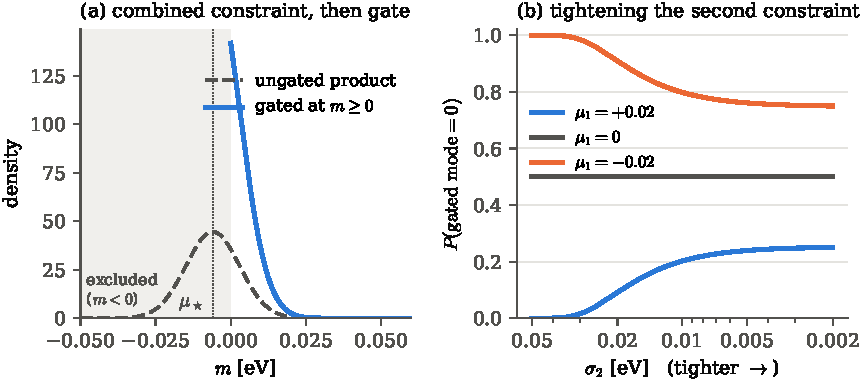
\includegraphics[width=\linewidth]{figures/fig_toy_boundary.pdf}
  \caption{The two-constraint model. (a) With $\mu_1=0.05$, $\sigma_1=0.02$, $\mu_2=-0.02$ and $\sigma_2=0.01$\,eV, the ungated product (dashed) peaks at $\mu_\star=-0.006$\,eV. After the gate, the density (solid) has its mode at $m=0$ but no atom there. (b) Probability of a boundary mode, \cref{eq:sweep_probability}, as the second constraint tightens, for $\mu_1\in\{+0.02,0,-0.02\}$\,eV, $\sigma_1=0.02$\,eV, $d=0$ and $s=0.03$\,eV. Tightening raises the probability when $\mu_1>0$, lowers it when $\mu_1<0$, and leaves it unchanged when $\mu_1=0$.}
  \label{fig:toy}
\end{figure}

\subsection{The finite upper prior and the reading of upper limits}
Posteriors are computed with a finite prior box, here $\mnu\le5$\,eV. The next statement shows what such a box can and cannot hide.

\begin{proposition}[Finite upper gate]\label{prop:upper-gate}
Let $\nu$ be any probability law on $\mathbb{R}$ with CDF $F$ and $F(U)>0$. Conditioning on $m\le U$ gives the CDF $F_U(x)=F(\min(x,U))/F(U)$. For every $x$,
\[
  0\;\le\; F_U(x)-F(x)\;\le\; 1-F(U),
\]
with equality on the right at $x=U$. For the gated Gaussian of \cref{prop:law} and any $U>0$, each level $0<q<1$ has a unique conditioned quantile in $(0,U)$.
\end{proposition}

The error introduced by a finite upper gate is therefore bounded by the probability that the wider posterior assigns above $U$. That probability has to be established separately. A small conditional upper limit does not establish it. As an exact example, take a likelihood equal to $47/10$ on $[0,1/5]$, $3/50$ on $[5,6]$, and zero elsewhere. With a flat prior on $[0,5]$ its 95th percentile is $0.19$\,eV, while with a flat prior on $[0,6]$ it is $31/6\approx5.17$\,eV. We do not suggest that the real likelihood behaves like this. The example only shows why the absence of samples near $5$\,eV is not, by itself, a proof that the prior box is irrelevant.

\begin{proposition}[Comparing two upper limits]\label{prop:readout}
Let $q_A,q_B$ be two upper limits and $\hat q_A,\hat q_B$ their estimates, with $|\hat q_A-q_A|\le\varepsilon_A$ and $|\hat q_B-q_B|\le\varepsilon_B$. Then $|(\hat q_A-\hat q_B)-(q_A-q_B)|\le\varepsilon_A+\varepsilon_B$, and the bound can be attained. If $\hat q_A-\hat q_B>\varepsilon_A+\varepsilon_B$ then $q_A>q_B$. When the estimates are random variables on a common probability space, the probability that the combined bound fails is at most the sum of the two individual failure probabilities, whatever the dependence between the estimates.
\end{proposition}

\subsection{What the model does and does not say about the lens swap}
The model shows that a hard gate can turn a nonpositive combined mean, for example from a moderate negative pull, into a mode at exactly zero, and that whether tightening favors this depends on the sign of the other constraint. It does not show that the SPT lens swap creates such a pull. Nor does it show that the real posteriors are Gaussian or that their constraints are independent. Our own sampled posteriors cannot settle the question (\cref{sec:results-mnu}). The model's practical lesson is about reporting. When the posterior sits against the gate, quantiles of the gated law (\cref{prop:law}) remain meaningful. The location of the mode, in contrast, can switch to or away from zero under modest changes in a constraint's mean.

\section{Discussion}
\label{sec:discussion}

\subsection{What the audits tell us}
The SPT 2018 and D1 likelihoods do not predict each other well. At the audited fits, parameters chosen by one lens cost the other tens to hundreds of units of $\chi^2$, and the cost depends strongly on direction: testing D1 at a 2018 fit is always the more expensive transfer. Extra D1 multipole coverage, the two releases' different optical-depth priors and default Boltzmann precision change these numbers by a few percent at most. Re-fitting a capped set of nuisance parameters absorbs a large share of the fixed-spectrum disagreement, but not all of it. Where the disagreement sits depends on what else is in the fit. Temperature at $2000\le\ell<3000$ leads both directions with SPT and DESI. Polarization leads the D1-given-2018 direction once the Planck subset and PR4 lensing are added.

Read through the SBT lens, the $\mnu$ shift reported in \cite{arxiv2601_16277} is a change of package under a lens swap, and the two lenses disagree at the level of the packaged likelihoods themselves. Until that disagreement is understood, a shift in a tight limit should be regarded as sensitive to packaging. This conclusion does not depend on the size of the shift, and it does not imply that either release is wrong.

\subsection{Limitations}
\begin{itemize}[leftmargin=*, itemsep=2pt]
  \item \textbf{Optimization.} All audit values are differences between numerically optimized candidates without a global-optimality certificate. Improved source fits moved individual values by up to a few percent. The positivity of $\dchi$ is guaranteed only between the retained candidates.
  \item \textbf{Significance.} The two releases differ in seasons, noise and nuisance models. Without a declared null distribution the $\dchi$ values are comparative diagnostics, not $p$-values. Signed allocations are not independent chi-squares.
  \item \textbf{Nuisance scope.} The SPT+DESI audits and chains fix SPT nuisance parameters at packaged defaults. The full baseline frees only three, and the fixed-spectrum audit re-fits a capped set of twelve. Broader nuisance freedom could change both the audit values and the posteriors.
  \item \textbf{Baseline scope.} Our full baseline omits SPT lensing and differs from the SPT+DESI baseline in Boltzmann code and free foregrounds. Comparisons between the two baselines do not isolate a single cause.
  \item \textbf{Posteriors.} We have no converged $\mnu$ posterior on a qualified numerical target (\cref{sec:results-mnu}). The likelihoods' sensitivity to solver version, caching and precision settings is part of the reason.
  \item \textbf{Released objects only.} The audits operate on released likelihoods. They say where the packaged summaries disagree, not whether calibration, beams, transfer functions, foreground modeling, map-making or covariance construction is responsible.
\end{itemize}

\subsection{Next diagnostics}
The decisive test remains the one proposed in \cite{arxiv2601_16277}: reprocess the 2018 raw data through the D1 pipeline. Short of that, three steps follow from this work.
\begin{enumerate}[leftmargin=*, itemsep=2pt]
  \item \textbf{Predictive audits.} Replace best-fit transfer with posterior predictive checks across lenses \cite{gelman_meng_stern1996_ppc}, with a declared null that accounts for differing noise and seasons. This would turn the localization maps into calibrated statements.
  \item \textbf{Controlled targets.} Fix and record the solver version, precision settings and caching behavior. Verify stored chain rows against fresh evaluations. Only then sample to the quantile precision required by \cref{prop:readout}, given the size of the shift to be resolved.
  \item \textbf{Targeted rewrites.} Where the mismatch localizes (EE at $2000\le\ell<3000$ in the full baseline, TT in the same range with SPT and DESI), test small template or calibration corrections fitted on one lens and evaluated on the other. A correction selected to fit the residual it removes improves the fit by construction. Its value must be judged on held-out data.
\end{enumerate}

\subsection{Practical recommendation}
When a likelihood update moves a tight bound, we suggest reporting, alongside the bound: the directional mismatch in both directions; its signed, covariance-respecting localization by spectrum and multipole, for each baseline used; at least one support control; and posterior diagnostics with quantile-precision targets matched to the size of the claimed shift. These are inexpensive compared with the inference itself, and they change how a moving bound should be read.

\section{Conclusion}
\label{sec:conclusion}

We analyzed the ``curious'' $\mnu$ sensitivity to the SPT-3G 2018$\rightarrow$D1 likelihood swap highlighted by \cite{arxiv2601_16277} through the Six Birds / SBT lens \cite{sixbirds_foundations,sixbirds_darkenergy}. Treating likelihood releases as distinct lenses, we provided reproducible directional audits, localization by spectrum and multipole, and a common-staging control. The mismatch is large, directional, and dominated by TT high-$\ell$ structure inside the overlap region; restricting D1 to the SPT2018 multipole support does not resolve it. We also reproduced the direction of DESI-driven $\mnu$ tightening under the lens swap and clarified why boundary motion can arise generically under a hard physical gate.

Our central message is methodological: when a parameter bound moves under a lens swap, the appropriate response is to report (and interpret) the bound together with lens-swap audits and staging controls. Doing so turns an ambiguous ``tension'' into an actionable diagnosis and provides a disciplined path toward resolving packaging instabilities without prematurely attributing them to new cosmology.


\bibliographystyle{unsrt}
\bibliography{references}

\end{document}
